\documentclass{article}
\usepackage[utf8]{inputenc}
\usepackage[american]{babel}
\usepackage{csquotes}
\usepackage{hyperref}
\usepackage[backend=biber,style=numeric,hyperref=true,natbib=true,autocite=plain,sorting=none]{biblatex}

\addbibresource{references.bib}

\title{%
	An Analysis of the Indian \textit{Areca} Fruit Husk (\textit{Areca Catechu L.}) as an Alternate for Polyester Fibers \\
	\large E344 – Knowledge Advancement Project}

\date{October 2018}
\author{Joshua Schmidt }

\usepackage{graphicx}

\begin{document}

\maketitle
\section{Abstract}

Synthetic fibers are found in nearly every piece of clothing and textile produced today \autocite{ihsmarkit}. These fibers have seen a meteoric rise in popularity due to their superior strength and material properties in comparison to traditional natural fibers \autocite{craftechindustries}. However, these synthetic fibers are non-renewable, and contribute to a significant amount ($>$25\%) of the microplastics found in the world's oceans \autocite{quantifyingfibers}\autocite{noaamicroplastics}. In order to combat the prevalence of synthetic fibers, many natural fiber alternatives are explored, comparing the material properties of these fibers to their synthetic counterparts \autocite{naturalfiberreview}. A feasibility analysis was completed to determine which natural fibers would most likely be used to replace synthetic fibers, and which natural fibers would have the most impact on the industry. It was determined that Indian Areca fruit husk fibers (Areca Catechu L.) (AFH) would be the most impactful natural fiber, as this fiber has superior material properties to the most prevalent synthetic fiber produced today - polyester \autocite{afhfiber}. AFH is already being produced in large quantities in the tobacco industry, but adapting this natural fiber can potentially have initial costs for the necessary processing infrastructure \autocite{afhfiber}. The difficulties of using this natural fiber, and the differences in material and molecular properties, were explored in this paper.

\section{Introduction}

Typically the main focus of renewable and sustainable living is energy production, for use at home, at work, and for transportation. The energy sector is seeing an unprecedented shift from non-renewable sources of energy to renewable ones, which is amazing for the world and for the environment. However, people typically fail to recognize the carbon footprint of the products they buy, especially those that are necessities. Clothing is one such product, stealthily releasing carbon into the environment every time it is washed. Small microfibers wear off of the synthetic textiles, entering waterways and wreaking havoc on marine ecosystems.

The international garment industry is massive, valued at over 780 billion USD in 2018 \autocite{shenglufashion}. It is expected to grow at an average of 4.3\% for the next five years, with average consumption per person increasing at that same rate \autocite{shenglufashion}\autocite{grandviewresearch}. With such a large global market size and excess production, garment and textile prices are very low - so low that the world consumes an estimated 80 billion textiles each year \autocite{shenglufashion}\autocite{grandviewresearch}. This number of textiles massively outweighs the less than 7.5 billion people alive today by a factor of 10, per year\autocite{grandviewresearch}.

The ubiquity of garments and textiles means that nearly every person throughout the world has access to clothes. But it also creates large environmental problems. The average American throws away 70 pounds of clothing each year, equivalent to more than 200 men's T-shirts, and most of these garments end up in landfills \autocite{shenglufashion}\autocite{grandviewresearch}. Eventually, these garments decay and break down, releasing their fibers into the environment. In 2016, approximately 63\% of fibers used in making textiles were made of synthetic materials \autocite{ihsmarkit}. These synthetic fibers take much longer to degrade than similar biodegradable materials - on average 30 years longer \autocite{ihsmarkit}. Additionally, when these synthetic fibers break down due to weathering and water saturation, they form microfibers \autocite{quantifyingfibers}. Microfibers are a form of microplastics that are created from synthetic fibers \autocite{quantifyingfibers}.

Microplastics, typically less than 5mm long, are extremely harmful to ocean and aquatic life, endangering thousands of species of fish, algae and other aquatic life \autocite{gesamp}. These plastics are the most prevalent form of marine debris found in our oceans and fresh water lakes, at over 146 thousand metric tons \autocite{noaamicroplastics}\autocite{iucn}. And microplastics are extremely difficult, if not impossible, to remove from large bodies of water \autocite{noaamicroplastics}. Currently, international entities such as the European Union and United Nations have created guidelines to reduce the use of plastics in everyday products, and recognize the growing microplastic problem \autocite{iucn}. But there are few programs, if any, to remove microplastics from the oceans due to the difficulty of the problem \autocite{iucn}. The polymers used in plastics and synthetic fibers are difficult to remove or break down due to their chemical bonding properties, which is good for the durability of the products they create, but terrible for the environment \autocite{microplasticrelease}. Every time garments made with synthetic fibers are washed, hundreds of microfibers are released into the water \autocite{microplasticrelease}. When considering every garment that is washed per person per year, this results in excess of 20 kilotons of microfibers produced per year globally, as a conservative estimate \autocite{microplasticpollutionlitreview}. With such high use of synthetic fibers in the textile industry and the large amount of microfibers produced each year, new materials are needed with the same benefits as synthetic fibers, but without the environmental detriments.

\section{Specific Product-Related Problem}
There are many different types of fibers used in the garment industry, with Nylon, Polyester, Wool, and Cotton being the most commonly used \autocite{naturalfiberreview}. They are generally split into two categories - synthetic and natural fibers \autocite{naturalfiberreview}\autocite{comparisonsyntheticfibers}. Natural fibers fall into two sub-categories - protein based (such as wool and silk) and cellulose based (such as cotton) \autocite{comparisonsyntheticfibers}. Both of these types of natural fibers have an affinity for water. Synthetic fibers, with the exception of some high-performance fibers (like Kevlar and Vectran), generally have much simpler molecular structures than the natural fibers \autocite{comparisonsyntheticfibers}. There are therefore numerous property consequences, including moisture absorption and response to mechanical stress \autocite{polyesterstrength}. The synthetic fibers can also be divided into subcategories - polyolefin (polypropylene, polyethylene), polyamide (nylon), and polyester \autocite{comparisonsyntheticfibers}. In the order stated, the strength of the fibers is increasing, as is their stiffness \autocite{polyesterstrength}. Polyolefin fibers typically have low moisture absorption, with nylon being somewhat higher, but not nearly at the same level as natural fibers \autocite{naturalfibercompositereview}.

\begin{figure}
  \centering
  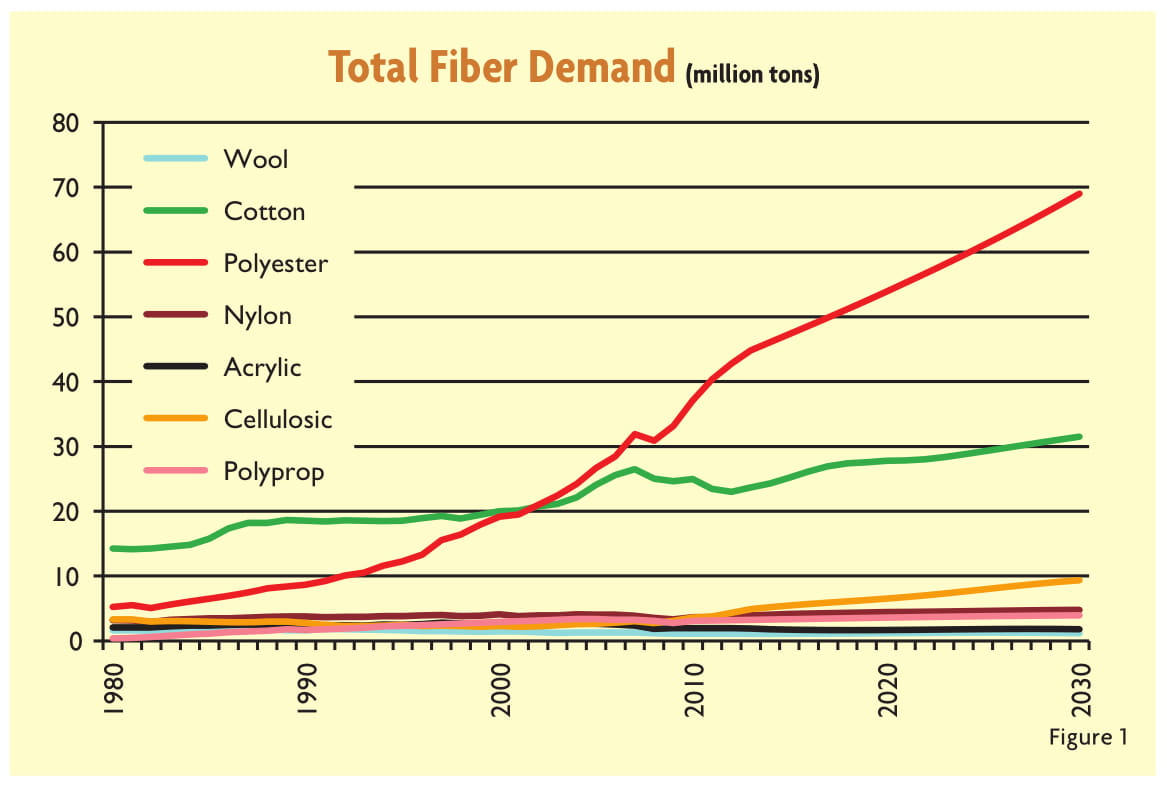
\includegraphics[width=0.5\textwidth]{assets/polyester_rise.jpg}
  \caption{Increasing use of Synthetic Fibers \protect\autocite{globaltradeanalysis}}
  \label{fig:syntheticfiberuse}
\end{figure}

Currently, polyester is the most used fiber in the United States, with approximately 60\% of the fiber market, or 50 million metric tons produced per year \ref{fig:syntheticfiberuse}\autocite{globaltradeanalysis}. Polyester is being used more and more year-over-year, as the demand for garments far outpaces the world's cotton and natural fiber production capacity \autocite{globaltradeanalysis}. The most effective way to combat the rise of synthetic fibers would therefore be to find a suitable alternative to polyester - a fiber that is biodegradable and natural, and yet has the same if not superior properties to polyester \autocite{naturalfiberprogressreport}. Additionally, this fiber needs to be available in large quantities, to meet the demand of an increasing world population, with room to scale dynamically \autocite{grandviewresearch}. The currently most popular natural fibers are not suitable to replace polyester as evidenced by polyester's meteoric rise in popularity \ref{fig:syntheticfiberuse}.

Polyester is made of long-chain polymers \autocite{polyesterstrength}. There are two main types of polyester - polyethylene terephthalate (PET) and poly-1,4-cyclohexylene-dimethylene (PCDT) \autocite{polyesterstrength}. PET is more popular since it can be used in a varietyof different products \autocite{polyesterstrength}. PET is also stronger than PCDT \autocite{craftechindustries}. However, PCDT is more elastic and resilient, making it suitable for more rugged products \autocite{polyesterstrength}. Being an ester, polyester is formed from an acid - benzene-1,4-dicarboxylic acid (terphthalic acid), and an alcohol, ethane-1,2-diol \autocite{polyesterstructure}.

\begin{figure}
  \centering
  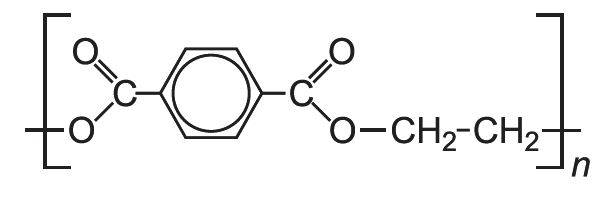
\includegraphics[width=0.5\textwidth]{assets/polyester_structure.jpg}
  \caption{Structure of Polyester \protect\autocite{polyesterstructure}}
  \label{fig:polyesterstructure}
\end{figure}

Polyester is made using a chemical reaction involving petroleum, air, water and coal \autocite{craftechindustries}. The most common process takes place at high temperatures in a vacuum \autocite{craftechindustries}. A petroleum by-product - alcohol - and carboxyl acid are mixed together, forming a monomer compound or "ester", through a reaction known as polymerization \autocite{polyesterstrength}. The polymer material created during polymerization is extruded while cooling into long fibers stretched to approximately five times their original length \autocite{craftechindustries}. The resulting fiber and its molecular structure is very strong \autocite{polyesterstrength}. These fibers are then used in a spinning process to make stronger threads that can then be used in textile manufacturing \autocite{craftechindustries}.

Polyester is an ideal fiber to use in garments and textiles due to its following properties: high strength, resiliency, resistance to most chemicals, quick drying, washability, resistance to mildew, resistance to wrinkles, and crease retention \autocite{craftechindustries}. These superior properties, and the relatively inexpensive materials used in the manufacturing process, explain why polyester is used so much in the textile industry.

\section{Proposed Materials Solution}

Polyester has great material properties, but its manufacture is unsustainable. When polyester breaks down, it releases harmful inorganic molecules to the environment, including waterways and oceans \autocite{wastewaterbangladesh}. These inorganic molecules are chemically inert, which is good for the durability of polyester, but detrimental to the environment as a whole \autocite{polyesterstrength}\autocite{gesamp}. The best solution is to find a natural polymer - a biopolymer - that can be used instead of polyester in the fabrication of fibers used in the textile industry \autocite{gesamp}. Given time, a natural fiber can be used to replace polyester fibers altogether.

Natural fibers divide into three different categories - animal fibers, mineral fibers, and plant fibers \autocite{naturalfiberreview}. Animal fibers consist of wool, silk, and avian fiber, including sheep's wool, horse hair, feathers, and feathers fiber \autocite{naturalfiberreview}. Animal fibers will not be considered as viable alternatives to polyester because they typically cost 150-500\% more than similar quantities of polyester \autocite{naturalfiberreview}. Mineral fibers consist of ceramic, metal fibers and asbestos. There are no examples of mineral fibers that have similar properties to polyester \autocite{naturalfiberreview}. 

Plant fibers are the most promising category. These fibers are comprised mainly of cellulose, and can be further categorized into seed fibers, leaf fibers, skin fibers, fruit fibers, and stalk fibers \autocite{naturalfiberprogressreport}. Cotton, bamboo, bagasee, jute, flax, hemp, coir, kapok, stalk straw, broom root, abaca leaves, banana leaves, and sisal leavs are all plant fibers that are currently being used as alternatives to synthetic fibers in textiles \autocite{naturalfiberprogressreport}. They have similar or greater tensile strength (150-900 MPa) to polyester (120 MPa) \autocite{polyesterstrength}\autocite{naturalfiberreview}.

However, there is one plant fiber that is very promising. Specifically, the Indian Areca fruit husk fibers (Areca Catechu L.) (AFH) \autocite{afhfiber}. AFH is rich in fiber and cellulose, and is wasted in large quantities by the tobacco industry \autocite{afhfiber}. The tensile strength of AFH is higher than polyester, at 231.66 MPa, and it has a porous surface morphology (40.8\%), which ensures better bonding with the rest of the fiber matrix. The cellulose content of the fiber is 57.35wt\%, which is very high for a plant fiber \autocite{afhfiber}. And the density of the fiber is low at 0.78\%, making it an attractive alternative to polyester \autocite{afhfiber}. It has a great weight-to-strength ratio, is already being produced in large quantities, and is completely biodegradable \autocite{afhfiber}. The fiber is also semi-crystalline, reducing the water absorption characteristics and making the material ideal for lightweight sports garments \autocite{afhfiber}. It can withstand temperatures of up to 240C, which is higher than the polymerization temperature of polyester \autocite{afhfiber}. AFH fibers are therefore a viable alternative to synthetic fibers like polyester. The material properties are similar or superior, the cost is relatively low compared to other potential natural fibers, and AFH is already being produced in large industries.

\begin{figure}
  \centering
  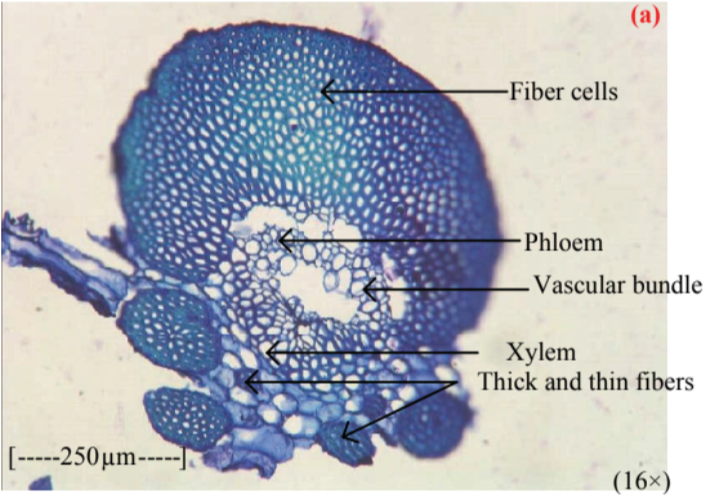
\includegraphics[width=0.5\textwidth]{assets/afh_fiber_structure.png}
  \caption{Inner Structure of AFH Fiber \protect\autocite{afhfiber}}
  \label{fig:afhstructure}
\end{figure}

\begin{figure}
  \centering
  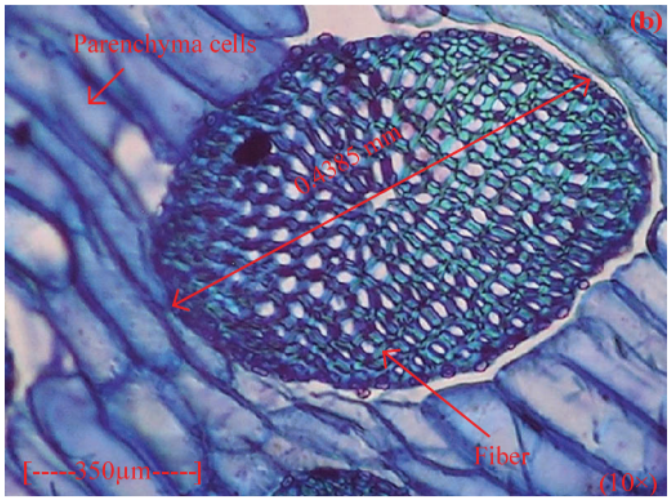
\includegraphics[width=0.5\textwidth]{assets/afh_fiber_top.png}
  \caption{AFH Fiber in matrix \protect\autocite{afhfiber}}
  \label{fig:afhinmatrix}
\end{figure}

\begin{figure}
  \centering
  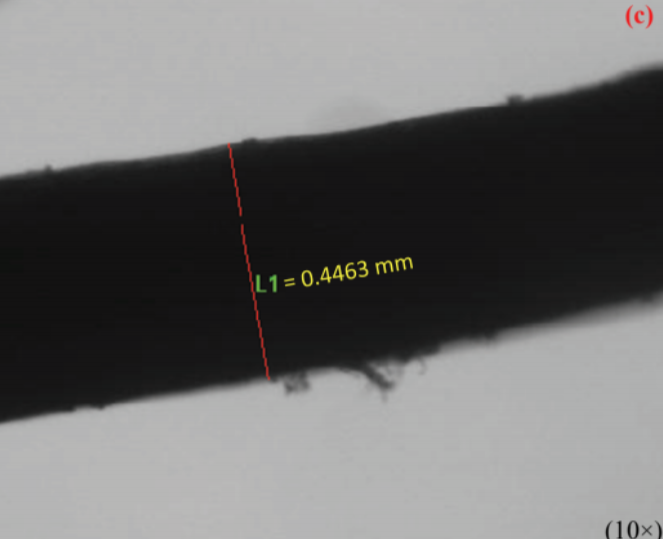
\includegraphics[width=0.5\textwidth]{assets/afh_fiber.png}
  \caption{AFH Fiber width \protect\autocite{afhfiber}}
  \label{fig:afhfiber}
\end{figure}

\begin{figure}
  \centering
  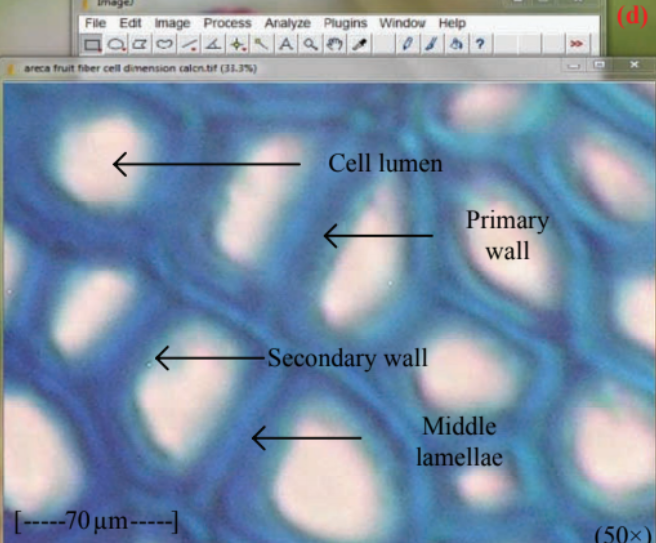
\includegraphics[width=0.5\textwidth]{assets/afh_cells.png}
  \caption{AFH Fiber Cells \protect\autocite{afhfiber}}
  \label{fig:afhcell}
\end{figure}

AFH has a very complex molecular structure that is difficult to fully describe and quantify. Its basic molecular elements are Cellulose (57.35-58.21 wt\%), Hemi cellulose (13-15.42 wt\%), Lignin (23.17-24.16 wt\%), wax (0.12 wt\%), and moisture (7.32 wt\%) \autocite{afhfiber}. It is therefore more rewarding to describe the fiber qualitatively, through the analysis of the figures shown above. Figure \ref{fig:afhstructure} shows a structural top view of AFH, with the various fiber cells, phloem, and different thicknesses inside the fiber \autocite{afhfiber}. The complex geometry of the cells in the fiber forms an nearly-crystalline structure with great tensile properties \autocite{afhfiber}. Looking at Figure \ref{fig:afhinmatrix}, the fibers are suspended in Parenchyma cells, which provides greater stability for the individual fibers \autocite{afhfiber}. Next Figure \ref{fig:afhfiber} shows one AFH fiber in a side-view, with a diameter of approximately 0.4463mm \autocite{afhfiber}. This diameter is relatively large in comparison to other . Figure \ref{fig:afhcell} shows the individual cells in an AFH fiber. The primary and secondary walls of the cells give the fiber its superior tensile strength characteristics \autocite{afhfiber}.

\section{Anticipated Challenges and Impact}

As the world shifts from nonrenewable to renewable forms of energy, the oil and petroleum industry is shrinking \autocite{iucn}. Less alcohol and ester is being produced as a byproduct of petroleum production \autocite{iucn}\autocite{craftechindustries}. However, the tobacco industry is large and growing despite the best efforts of governments around the world. AFH can be used to reduce the carbon footprint of the tobacco industry, and to make up for the lowering petroleum production worldwide \autocite{afhfiber}. If AFH can viably replace polyester as a major textile fiber, fewer synthetic fibers will turn into microplastics saturating the world's oceans \autocite{microplasticrelease}\autocite{gesamp}. As a biodegradable fiber, AFH will have little to no impact on marine life and the environment as a whole \autocite{gesamp}\autocite{afhfiber}. It will degrade much faster than polyester and other synthetic fibers, naturally breaking down into fundamental molecules \autocite{naturalfiberprogressreport}.

The first problem with using AFH is the increase in scale required to supply the world's textile industry with this material, so that it can compete with polyester \autocite{afhfiber}. While it is a good starting place that tobacco farms are producing the husks as a byproduct, a far greater manufacturing capacity is required to match the production of polyester \autocite{afhfiber}. One main advantage of polyester is that it does not require farm land to produce. With limited land and space available to grow AFH, one solution is to grow the material in vertical farms near city centers. With over 50\% of the world's population expected to live in or near cities by 2050, it makes sense to have the supply of AFH near consumers of the product \autocite{globaltradeanalysis}. Vertical farms, agile manufacturing and quick fashion turn-around can spell success for textile and garment companies using AFH.

However, the major problem with using AFH is the change in manufacturing infrastructure required to process and use this natural fiber \autocite{afhfiber}. The fruit husks will need to be shipped from tobacco farms to textile fiber manufacturing facilities, which will need to be completely retooled \autocite{afhfiber}. Advanced machines to clean and extract the fibers from the raw fruit husks are necessary, as well as new spindles to twist the fibers into thread. Natural fiber processing is currently quite varied in approach, with many private companies using proprietary methods to clean and process the fibers \autocite{afhfiber}. There is no industry standard, and no common method, for processing the many different natural fibers \autocite{afhfiber}. There is also no current published method for processing AFH fibers specifically. However, there are methods for processing Lignin and fibers with high cellulose concentrations, which is a category that AFH falls into \autocite{afhfiber}. But there is no industry standard method at the moment for doing so. All of these challenges can be overcome with an increase in capital and investment in the product \autocite{afhfiber}. However with the low margins in the textile industry, it will require a significant change in the consumer awareness and motivation to switch to AFH textiles.

What is far more likely is that economic forces will push the textile industry towards renewable fibers. As petroleum prices rise and renewable energy prices decline, polyester will become more expensive to produce until the Areca Fruit Husk or another natural fiber will be the cheaper option \autocite{afhfiber}. But until that point, it is expected that the textile industry will continue to use synthetic fibers like polyester, leading to thousands more metric tons of microplastics entering our oceans every year.


\printbibliography
\end{document}
